\documentclass[a4paper, 11pt]{article}
\usepackage[english]{babel}
\usepackage[utf8]{inputenc}
\usepackage{amsmath}
\usepackage{graphicx}
\usepackage{float}
\usepackage{fixltx2e}
\usepackage{listings}
\usepackage{color}
\usepackage{latexsym}
\usepackage{lstautogobble}
\usepackage[colorinlistoftodos]{todonotes}
\usepackage[margin=3cm]{geometry}
\usepackage{hyperref}
\usepackage{libertine}
\usepackage{tikz}
\hypersetup{
	hidelinks, 
	colorlinks = true,
	linkcolor = black,
}

\usetikzlibrary{shapes, arrows}

\newtheorem{definit}{Definizione}[subsection]

\begin{document}
	\clearpage
	\begin{titlepage}
		\centering
		\vspace*{\fill}
		{\scshape\LARGE Università degli Studi di Verona \par}
		\vspace{1.5cm}
		\line(1,0){150} \\
		{\huge\bfseries Crittografia\par}
		\line(1,0){150} \\
		\vspace{0.5cm}
		{\scshape\Large Riassunto dei principali argomenti\par}
		\vspace{2cm}
		{\Large\itshape Davide Bianchi\par}
		\vspace{1cm}
		\vspace{5cm}
		\vspace*{\fill}
		% Bottom of the page
		{\large \today\par}
	\end{titlepage}
	\thispagestyle{empty}
	\newpage
	\tableofcontents
	\newpage
	
	\section{Introduzione}
	Iniziamo dando alcune definizioni fondamentali. Si useranno i termini \textit{ciphertext} e \textit{plaintext} per indicare rispettivamente il testo cifrato e quello in chiaro.
	
	\begin{definit}[Crittografia]
		Insieme dei metodi per rendere un messaggio non leggibile ad altri.
	\end{definit}
	
	\begin{definit}[Steganografia]
		Insieme dei metodi per nascondere l'esistenza di un messaggio in un altro contenuto.
	\end{definit}
	
	\begin{definit}[Crittoanalisi]
		Analisi del ciphertext per ottenere il plaintext corrispondente.
	\end{definit}
	
	Un generico sistema crittografico è strutturato come: \\
	
	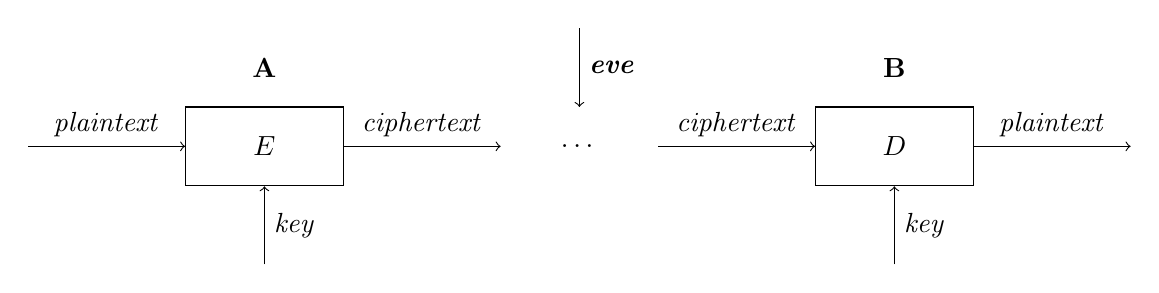
\begin{tikzpicture}
		\node at (4,0) [rectangle,draw, minimum width=2cm, minimum height=1cm] (E) {$E$};
		\draw (E);
		\draw[->] (1,0) -- (E) node[above, midway] {\textit{plaintext}};
		\draw[->] (4,-1.5) -- (E) node[right, midway] {\textit{key}};
		\draw[->] (E) -- (7,0) node[above, midway] {\textit{ciphertext}};
		\node at (8,0) (dots) {$\dots$};
		\node at (12,0) [rectangle,draw, minimum width=2cm, minimum height=1cm] (D) {$D$};
		\draw[->] (9,0) -- (D) node[above, midway] {\textit{ciphertext}};
		\draw[->] (12,-1.5) -- (D) node[right, midway] {\textit{key}};
		\draw[->] (D) -- (15,0) node[above, midway] {\textit{plaintext}};
		\node at (4,1) {\textbf{A}};
		\node at (12,1) {\textbf{B}};
		\draw[->] (8, 1.5) -- (8,0.5) node[right, midway] {\textbf{\textit{eve}}};
	\end{tikzpicture}
	
	dove:\begin{itemize}
		\item \textbf{A} e \textbf{B} sono i due enti che si devono scambiare il messaggio cifrato;
		\item \textbf{\textit{eve}} è un terzo che tenta di decrittare il messaggio;
		\item $E$ e $D$ sono i sistemi di \textit{encrypt} e \textit{decrypt};
		\item i 3 punti ($\dots$) rappresentano il mezzo impiegato per la trasmissione del messaggio (qualunque esso sia).
	\end{itemize}
	
	Ovviamente, per \textit{eve}, che tenta di decrittare il messaggio, non ha senso tentare di insistere se il costo della decrittazione è maggiore del valore dell'informazione da proteggere. In tal senso il sistema di cifratura è "sicuro". 
	
	La funzione $E$, inoltre, per essere sufficientemente affidabile, deve essere invertibile (in caso contrario non si potrebbe decrittare il messaggio), ma deve essere difficile fare ciò (in tal caso si dice che $E$ è una \textit{one-way function}). Con la chiave la funzione diventa facile anche da invertire (\textit{one-way trapdoor}).
	
	\section{Cifrari di base}
	\subsection{Cifrario di Cesare}
	Il messaggio viene cifrato sostituendo ogni lettera $l$ del messaggio con la $l+k$ esima lettera dell'alfabeto; la chiave quindi è data dalla coppia $(l, l+k)$. 
	
	Il cifrario di Cesare è facile da attaccare in quanto basta un attacco \textit{bruteforce}, quindi è sufficiente provare tutte le combinazioni (che sono in totale 26).
	
	\subsection{Permutazione casuale}
	Supponiamo di usare come cifrario una permutazione casuale dell'alfabeto, ovvero sostituendo ad ogni lettera dell'alfabeto un'altra lettera, in modo totalmente casuale. In tal caso l'attacco bruteforce richiederebbe tempo eccessivo (ci sono $26!$ pssibili combinazioni da provare, che sono decisamente troppe). 
	
	La tecnica usata per attaccare questo tipo di crittografia è l'\textit{analisi delle frequenze}, ovvero l'analisi delle lettere che capitano di più in una data lingua, e associare la lettera del messaggio cifrato con una data frequenza con quella nella lingua del messaggio con una frequenza simile.
	
	
	
	
	
\end{document}